\documentclass[11pt]{article}

\setlength{\oddsidemargin}{-0.25 in}
\setlength{\evensidemargin}{-0.25 in}
\setlength{\topmargin}{-0.9 in}
\setlength{\textwidth}{7.0 in}
\setlength{\textheight}{9.0 in}
\setlength{\headsep}{0.75 in}
\setlength{\parindent}{0.3 in}
\setlength{\parskip}{0.1 in}
\usepackage{epsf}
\usepackage{pseudocode}
\usepackage{amsmath}
\usepackage{amssymb}
\usepackage[normalem]{ulem}
\usepackage{graphicx}
\usepackage{color}
\usepackage[export]{adjustbox}
\pagenumbering{gobble}
\def\O{\mathop{\smash{O}}\nolimits}
\def\o{\mathop{\smash{o}}\nolimits}
\newcommand{\e}{{\rm e}}
\newcommand{\R}{{\bf R}}
\newcommand{\Z}{{\bf Z}}

\title{Section 2: Search Solutions}
\date{}
\author{CS 182 - Artificial Intelligence}
\begin{document}
\maketitle


\renewcommand{\labelenumii}{\arabic{enumii}.}
\setlength{\parindent}{0pt}

\begin{enumerate}

\item
% \emph{Review.} Consider the 8-puzzle, where tiles adjacent to blank spaces
% can slide into the blank spaces, until the puzzle is rearranged to fit the
% goal state. Describe each element of a search problem for solving this puzzle. (AIMA)
Consider the Tower of Hanoi puzzle, where a stack of disks
must be moved from the leftmost peg to the rightmost peg, while maintaining
the invariant that no disk may be placed on top of a smaller disk.
Describe each element of a
search problem for solving this puzzle. How many possible states are in
this representation? (Image: Popular Science Monthly Vol. 26)

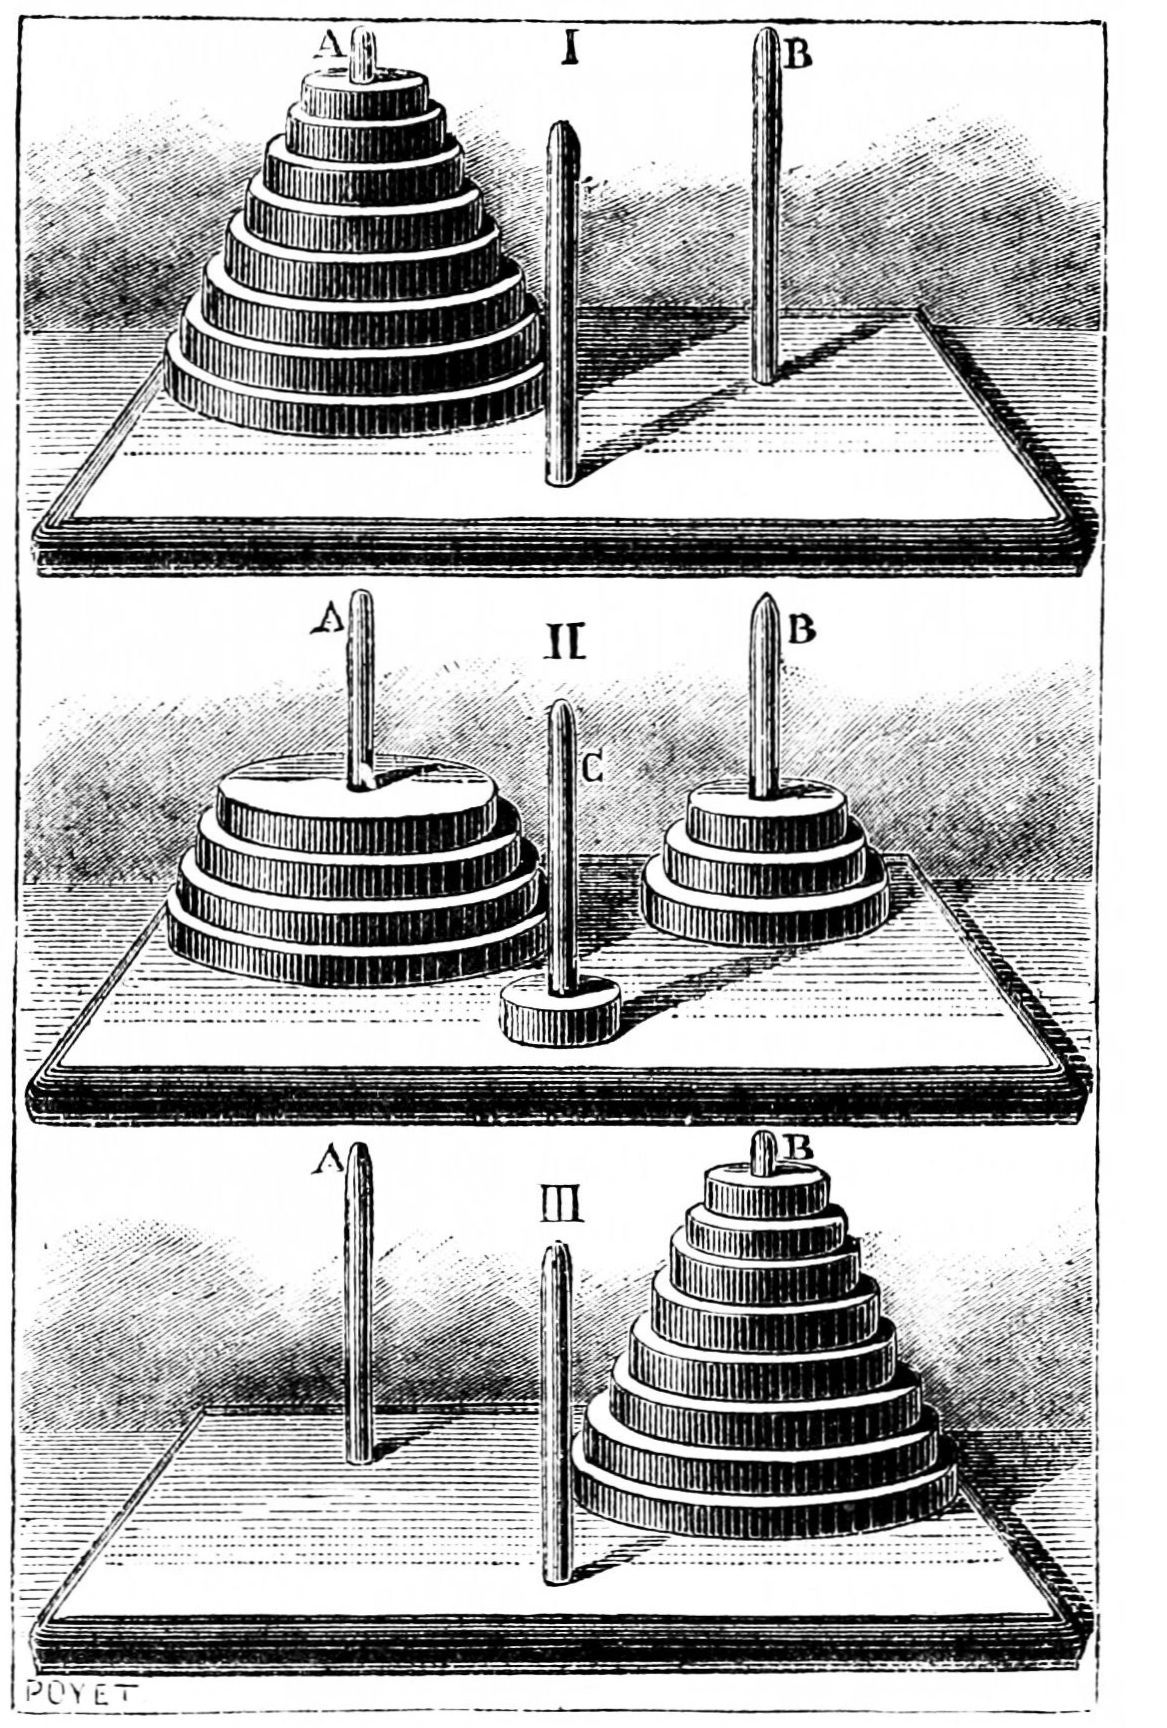
\includegraphics[scale=0.15, right]{img/hanoi}

\begin{itemize}
\color{blue}
\item $S:$ A state in this problem is a representation of which peg each disk lies on.
This can be thought of as an array mapping rings $1, 2, \dots, N$ to
pegs $1, 2, 3$, e.g. $[3, 2, 1, 3, 1, 2]$. Only one legal configuration is possible
for each arrangement of rings on a peg, because the rings can only be legally
ordered from smallest to largest.
Therefore, number of possible states is the number of possible mappings
of $N$ rings onto three pegs, which is \boxed{3^N}
\item $A:$ Legal actions are movement of the top ring on any peg to another peg
where all rings are larger than the ring being moved. Note that
the set of legal actions depends on the state.
\item $R:$ The transition model takes an initial state and action, and
returns the new state with a ring moved to another peg.
\item $C:$ As no one action is more costly than another, the cost for each
action is $1$.
\item $S_0:$ The starting state is the arrangement of $N$ rings on the leftmost peg
from smallest to largest.
\item $G:$ The goal test is whether the state is the arrangement of $N$
rings on the rightmost peg from smallest to largest.
\end{itemize}


\newpage
\item
Consider the 8 queens puzzle, where queens must be placed on a
chessboard so they do not attack each other. Describe each element of a
search problem for solving this puzzle. How many possible states are in
this representation? (AIMA)

\begin{figure}[h!t]
  \centering
  \caption{A nearly-complete 8-queens puzzle solution}
  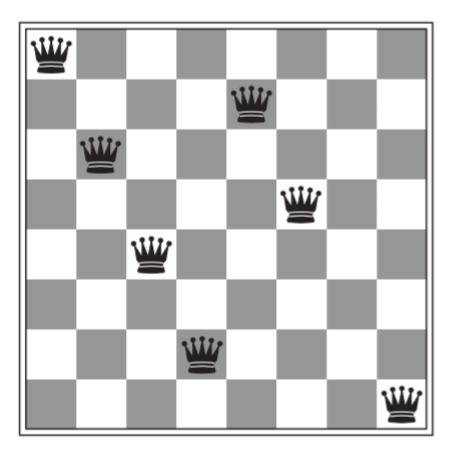
\includegraphics{img/8queens}
\end{figure}

\begin{itemize}
\color{blue}
\item $S:$ A state in this problem could be any arrangement of $0$ to $8$
queens on the chessboard. The number of possible states in this representation
is $\sum_{k=0}^8 \frac{64!}{(64-k)!} \approx 1.8 \times 10^{14}$
\item $A:$ Add a queen to an empty square if there are
fewer than $8$ queens.
\item $R:$ The transition model would return a board with a queen
added to the designated square.
\item $C:$ As no one action is more costly than another, the cost for each
action is $1$.
\item $S_0:$ The starting state is the empty board.
\item $G:$ The goal test is whether there are $8$ queens on the board
which do not attack one another.
\end{itemize}

\item Can you think of another, more compact representation of the state space? (AIMA)
\begin{itemize}
\color{blue}
\item $S:$ All possible arrangements of $k$ queens $(0 \le k \le 8)$,
one per column in the leftmost $k$ columns, with no queen attacking another.
AIMA lists the size of this state space as $2057$.
\item $A:$ Add a queen to any square in the leftmost empty column such that
it is not attacked by any other queen.
\end{itemize}

\newpage
\item
You are programming a holiday shopping robot that will drive from store to
store in order to buy all the gifts on your shopping list.  You have a set
of $N$ gifts $G = \{ g_1 ,g_2 ,...g_N \}$ that must be purchased.  There are
$M$ stores, $S = \{ s_1 ,s_2 ,...s_M \}$ each of which stocks a known inventory
of items:  we write $g_k \in s_i$ if store $s_i$ stocks gift $g_k$. Shops may
cover more than one gift on your list and will never be out of the items they
stock.  Your home is the store $s_1$, which stocks no items.

The actions you will consider are travel-and-buy actions
in which the robot travels from its current location $s_i$ to another
store $s_j$ in the fastest possible way and buys whatever items remaining on
the shopping list that are sold at $s_j$.  The time to travel-and-buy from
$s_i$ to $s_j$ is $t(s_i,s_j)$.  You may assume all travel-and-buy actions
represent shortest paths, so there is no faster way to get between
$s_i$ and $s_j$ via some other store.  The robot begins at your home with no
gifts purchased.  You want it to buy all the items in as short a time as
possible and return home.

For this planning problem, you use a state space where each state is a pair
$(s,u)$ where $s$ is the current location and $u$ is the set of unpurchased
gifts on your list (so $g \in u$ indicates that gift $g$ has not yet been purchased).
(Berkeley CS 188, Fall 2011)

How large is the state space in terms of the quantities defined above?

{\color{blue}
$M \times2^N.$
You are in one of
$M$
places (simple index from $1$ to
$M$), and have not purchased some subset of
$N$
items (binary vector of size
$N$).}

~\\ \\ \\ \\ \\ \\ \\

\item You have waited until very late to do your shopping, so you decide to send an swarm of
$R$ robot minions to
shop in parallel.  Each robot moves at the same speed, so the same
store-to-store times apply.  The problem
is now to have all robots start at home, end at home, and for each item
to have been bought by at least one
robot (you don’t have to worry about whether duplicates get bought).
Hint:  consider that robots may not all
arrive at stores in sync. (Berkeley CS 188, Fall 2011)

Give a minimal state space for this search problem:

{\color{blue}
We  need  the  location  of  each  robot  at  each  time.
At  a  given  time,  a  robot  can  either  be  at  one  of
$M$
stores, or in any of $(T ~- − 1) \cdot M$
transition locations, where
$T$
is the maximum travel distance between
two stores.  Thus, the location of each robot takes $(MT)^R$.
We also need the set of items purchased $(2^N)$.
Therefore, the size of each state is:  $(MT)^R\times 2^N.$}

\newpage
\item Consider the search graph shown below.
$S$ is the start state and $G$ is the goal state. All edges are bidirectional.
For each of the following \underline{graph} search strategies, give the path that would be returned,
or write none if no path will be returned. If there are any ties,
assume alphabetical tiebreaking (i.e., nodes for states earlier in the
alphabet are expanded first in the case of ties). (Berkeley CS 188, Fall
2011)

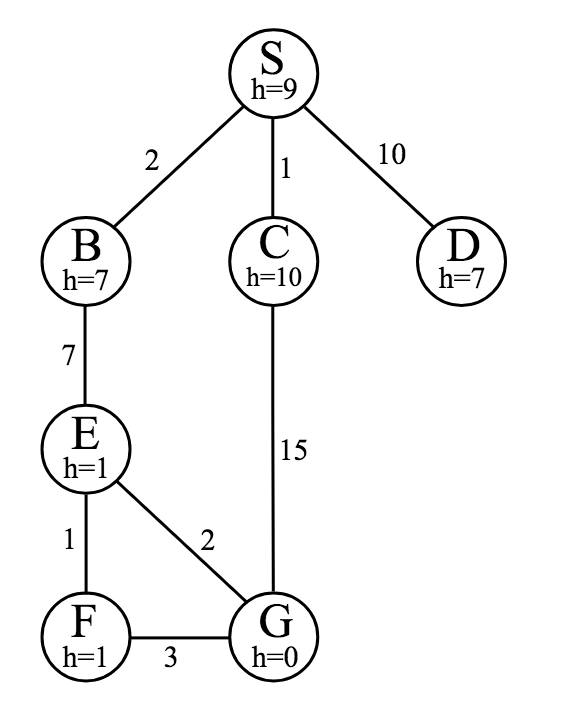
\includegraphics[scale=0.7, center]{img/tree2}

\begin{itemize}
\item DFS
{\color{blue} S \rightarrow B \rightarrow E \rightarrow F \rightarrow G}

\bigskip
\bigskip
\item BFS
{\color{blue} S \rightarrow C \rightarrow G}

\bigskip
\bigskip
\item UCS
{\color{blue} S \rightarrow B \rightarrow E \rightarrow G}

\bigskip
\bigskip
\item Greedy Search
{\color{blue} S \rightarrow B \rightarrow E \rightarrow G}

\bigskip
\bigskip
\item A* Search
{\color{blue} S \rightarrow B \rightarrow E \rightarrow G}

\end{itemize}

\newpage
\item
Consider the state space graph shown below in which some of the states are
missing a heuristic value.  \\(Berkeley CS 188, Spring 2015)


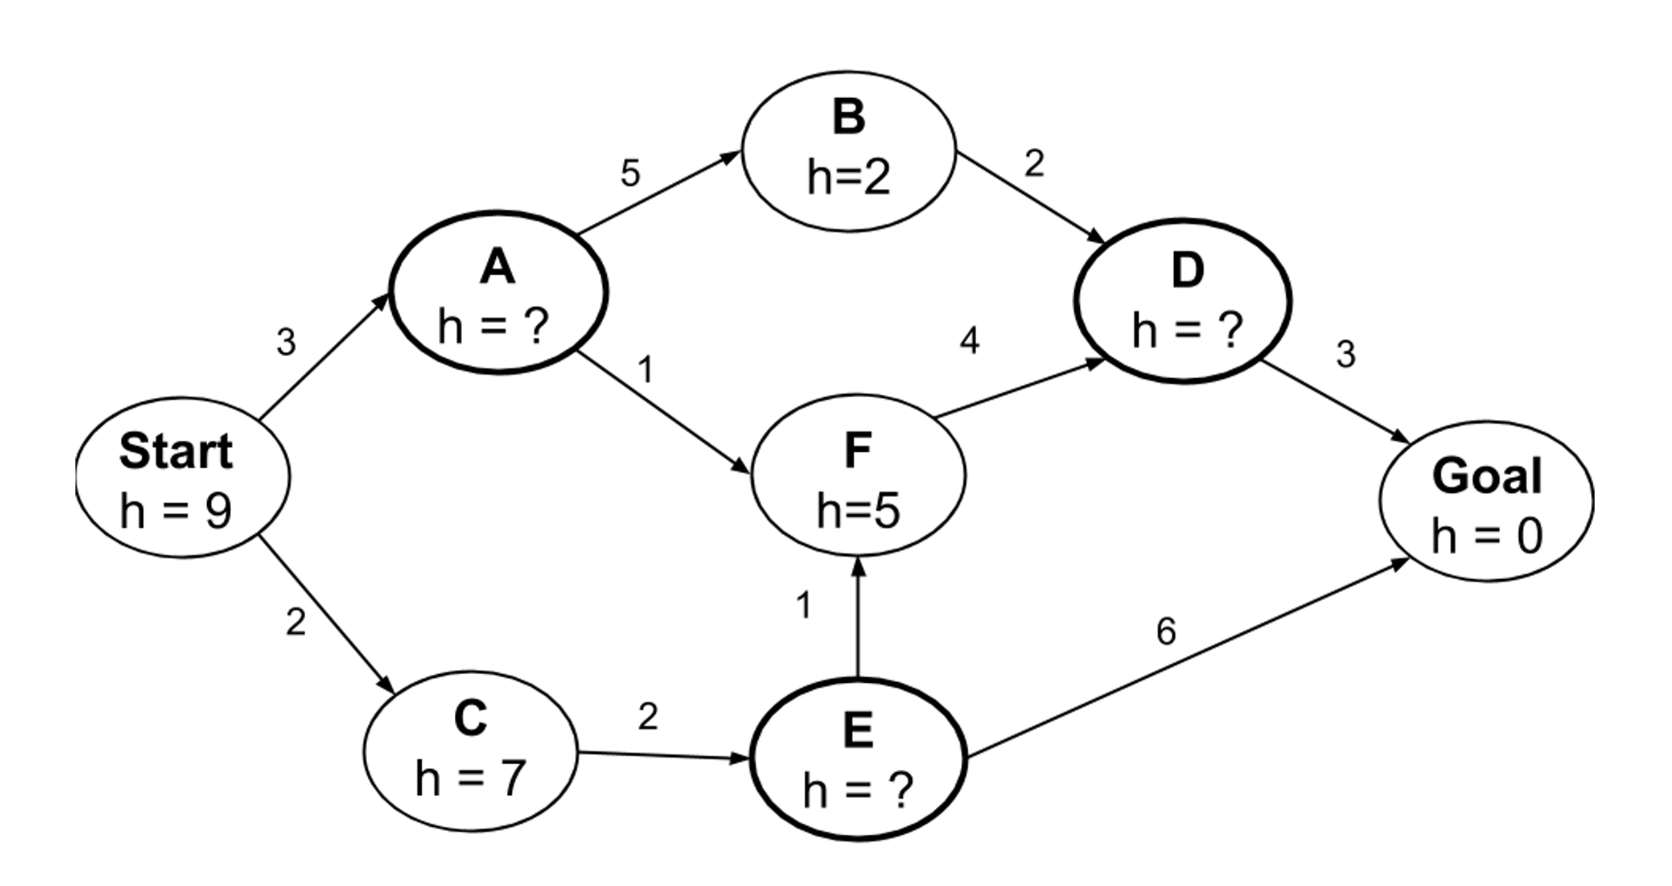
\includegraphics[width=\textwidth]{img/Heuristics}

Determine the possible range for each missing heuristic value so that the heuristic is admissible. 
~\\
\begin{enumerate}
\color{blue}
\item $h(A) \le 8$

\item $h(D) \le 3$

\item $h(E) \le 6$
\end{enumerate}
~\\ \\
Additionally, for what range of each heuristic value is the heuristic consistent? 
~\\
\begin{enumerate}
\color{blue}
\item $6 \le h(A) \le 6$
\item $1 \le h(D) \le 3$
\item $5 \le h(E) \le 6$

\end{enumerate}

\newpage
\item
The heuristic path algorithm (Pohl, 1977) is a best-first search in which the evaluation
function is $f(n) = (2 ~ -w)g(n) + wh(n)$. (AIMA)

For what values of $w$ is this optimal, assuming that $h$ is admissible?

{\color{blue}
Divide by $(2 - w)$ to scale $f$ to $f'(n) = g(n) + \frac{w}{2 - w}h(n)$,
which is A* if $\frac{w}{2 - w} = 1$

To guarantee $h$ remains admissible after scaling, it cannot be scaled up,
(i.e. $\frac{w}{2 - w} \le 1$), since
scaling $h$ up may overestimate the distance to goal.

Therefore, this search is optimal if $w \le 1$.}
\\ \\
What kind of search does this perform for $w = 0$, $w = 1$, and $w = 2$?

{\color{blue}
$w = 0$: UCS

$w = 1$: A*

$w = 2$: Greedy} 
\\ \\ \\ \\ \\ \\

\item
For the Tower of Hanoi puzzle from before, come up with an admissible
heuristic function.

{\color{blue}
$h(n) = (\# \text{disks not on right peg}) + 2 \cdot
(\# \text{disks on right peg which are smaller than disks
not on right peg})$

This is an admissible heuristic because all disks not on the right peg must
be moved to the right peg, and any disk on the right that is smaller than a disk
on the middle or left must be moved away (to make room for the larger disk)
and then moved back.
}
\end{enumerate}

\newpage


\clearpage
\clearpage
\end{document}
